\documentclass[aspectratio=169, 10pt]{beamer}

% ── Theme & Colors ──────────────────────────────────────────────
\usetheme{Madrid}
\usecolortheme{default}
\definecolor{darkblue}{RGB}{0,51,102}
\definecolor{lightblue}{RGB}{51,122,183}
\definecolor{darkgreen}{RGB}{34,139,34}
\definecolor{highlight}{RGB}{220,50,47}
\setbeamercolor{structure}{fg=darkblue}
\setbeamercolor{frametitle}{bg=darkblue, fg=white}
\setbeamercolor{block title}{bg=lightblue, fg=white}
\setbeamercolor{block body}{bg=lightblue!10}
\setbeamercolor{block title alerted}{bg=highlight, fg=white}
\setbeamercolor{block body alerted}{bg=highlight!10}
\setbeamertemplate{navigation symbols}{}
\setbeamertemplate{footline}[frame number]

% ── Packages ────────────────────────────────────────────────────
\usepackage{amsmath, amssymb, amsthm}
\usepackage{mathtools}
\usepackage{bm}
\usepackage{booktabs}
\usepackage{csquotes}
\usepackage{tikz}
\usetikzlibrary{arrows.meta, positioning, shapes.geometric, calc, decorations.pathreplacing}
\usepackage{graphicx}
\usepackage{xcolor}

% ── Macros ──────────────────────────────────────────────────────
\newcommand{\vx}{\mathbf{x}}
\newcommand{\vz}{\mathbf{z}}
\newcommand{\va}{\mathbf{a}}
\newcommand{\vb}{\mathbf{b}}
\newcommand{\vc}{\mathbf{c}}
\newcommand{\R}{\mathbb{R}}
\newcommand{\Bp}{\mathcal{B}_p}
\newcommand{\Bq}{\mathcal{B}_q}
\newcommand{\PP}{\mathcal{P}}
\DeclareMathOperator*{\argmin}{arg\,min}
\DeclareMathOperator{\proj}{proj}

% ── Title ───────────────────────────────────────────────────────
\title[CPP Counterfactuals]{%
  Certified Polyhedral Projection\\[4pt]
  for Counterfactual Explanations}
\subtitle{Generating Valid, Proximal, and Robust Counterfactuals\\via Preimage Approximation}
\author{Gabriele Pintus}
\date{\today}

\begin{document}

% ================================================================
\begin{frame}
  \titlepage
\end{frame}

% ================================================================
\begin{frame}{Outline}
  \tableofcontents
\end{frame}

% ================================================================
\section{Motivation \& Background}

% ----------------------------------------------------------------
\begin{frame}{What Are Counterfactual Explanations?}

Given a classifier $f: \R^d \to \R^L$ and a query $\vx_0$ classified as class $l$:

\begin{block}{Goal}
  Find $\vx' \in \R^d$ that is \textbf{classified as target class} $t \neq l$ and is \textbf{as close as possible} to $\vx_0$.
\end{block}

\bigskip

\textbf{Example (MNIST):} ``What minimal change turns a \textbf{digit 1} into a \textbf{digit 7}?''

\bigskip

\textbf{Desirable properties:}
\begin{enumerate}
  \item \textbf{Validity} -- guaranteed to be classified as the target class
  \item \textbf{Proximity} -- minimal distance to the original input
  \item \textbf{Plausibility} -- stays close to the data manifold
  \item \textbf{Robustness} -- remains valid under small perturbations
\end{enumerate}

\end{frame}

% ----------------------------------------------------------------
\begin{frame}{Limitations of Existing Approaches}

Standard gradient-based methods solve:
\[
  \vx' = \argmin_{\vz} \bigl\| \vx_0 - \vz \bigr\|_p + \lambda \cdot \mathcal{L}_{\text{target}}\!\bigl(f(\vz)\bigr)
\]

\begin{alertblock}{Problems}
\begin{itemize}
  \item \textbf{Non-convex landscape} $\Rightarrow$ local minima, no global optimality
  \item \textbf{No validity guarantee} $\Rightarrow$ counterfactuals may land near the decision boundary
  \item \textbf{No robustness certificate} $\Rightarrow$ tiny perturbations can flip the prediction
  \item \textbf{Out-of-distribution} $\Rightarrow$ adversarial artifacts, not meaningful changes
\end{itemize}
\end{alertblock}

\bigskip

\begin{center}
\textbf{Our approach:} replace gradient descent on a non-convex loss\\
with \textcolor{darkgreen}{\textbf{convex projection onto certified polytopes}}.
\end{center}

\end{frame}

% ================================================================
\section{The CPP Method}

% ----------------------------------------------------------------
\begin{frame}{Core Idea: From Non-Convex Search to Convex Projection}

\begin{block}{Key Insight}
  If we can decompose the target class preimage into a \textbf{union of convex polytopes}
  $\PP_1, \PP_2, \dots, \PP_N$ where the classifier is \emph{guaranteed} to predict class~$t$,
  then finding the counterfactual reduces to:
  \[
    \vx' = \proj_{\bigcup_i \PP_i}(\vx_0) = \argmin_{\vz \in \bigcup_i \PP_i} \bigl\|\vx_0 - \vz\bigr\|_2
  \]
\end{block}

\bigskip

\begin{itemize}
  \item Each individual projection $\proj_{\PP_i}(\vx_0)$ is a \textbf{convex QP} $\Rightarrow$ \textbf{global optimum}
  \item The overall nearest projection is found by comparing across all $\PP_i$
  \item \textbf{No gradient descent}, no local minima, no hyperparameter $\lambda$
\end{itemize}

\end{frame}

% ----------------------------------------------------------------
\begin{frame}{Two-Phase Architecture}

\begin{columns}[T]
\column{0.48\textwidth}
\begin{block}{Phase I: Atlas Construction (Offline)}
  For each training sample $\vc_i$ of class $t$:
  \begin{enumerate}
    \item Define $L_p$ ball $\Bp(\vc_i, \varepsilon)$
    \item Run \textbf{LiRPA} backward-mode bound propagation
    \item Obtain linear bounds $A_i, \vb_i$ such that:
      \[
        A_i \vx + \vb_i \leq f_t(\vx) - f_j(\vx) \;\;\forall j \neq t
      \]
    \item Store certified polytope:
      \[
        \PP_i = \bigl\{\vx : A_i \vx + \vb_i \geq \mathbf{0}\bigr\} \cap \Bp(\vc_i, \varepsilon)
      \]
  \end{enumerate}
  \medskip
  $\Rightarrow$ \textbf{Every point in $\PP_i$ is guaranteed class $t$}
\end{block}

\column{0.48\textwidth}
\begin{block}{Phase II: Counterfactual Query (Online)}
  Given query $\vx_0$:
  \begin{enumerate}
    \item Use \textbf{BVH} spatial index to prune candidates
    \item For each candidate polytope $\PP_i$, solve QP:
      \[
        \min_{\vz}\; \|\vz - \vx_0\|_2^2
      \]
      subject to:
      \begin{align*}
        A_i\vz + \vb_i &\geq \mathbf{0} \\
        \|\vz - \vc_i\|_p &\leq \varepsilon
      \end{align*}
    \item Return projection with \textbf{minimum distance}
  \end{enumerate}
  \medskip
  $\Rightarrow$ \textbf{Globally optimal among all polytopes visited}
\end{block}
\end{columns}

\end{frame}

% ================================================================
\section{LiRPA Certification}

% ----------------------------------------------------------------
\begin{frame}{LiRPA: Linear Relaxation based Perturbation Analysis}

\textbf{Goal:} For a neural network $f$ and an input region $\Bp(\vc, \varepsilon)$, find linear functions that \textbf{bound} the network output from below.

\bigskip

\begin{block}{One-vs-All Formulation}
We wrap the classifier with a constraint layer:
\[
  g_j(\vx) = z_t(\vx) - z_j(\vx) \quad \text{for all } j \neq t
\]
where $z_k(\vx)$ is the logit for class~$k$. The sample is classified as $t$ iff $g_j(\vx) \geq 0\;\forall j$.

\medskip

LiRPA computes \textbf{linear lower bounds}:
\[
  \va_{ij}^\top \vx + b_{ij} \leq g_j(\vx) \quad \forall\, \vx \in \Bp(\vc, \varepsilon)
\]

Therefore: $\va_{ij}^\top \vx + b_{ij} \geq 0 \;\Longrightarrow\; g_j(\vx) \geq 0 \;\Longrightarrow\; \text{class } t$ certified.
\end{block}

\bigskip

Stacking all $K{-}1$ constraint rows gives the matrix $A_i \in \R^{(K-1) \times d}$ and vector $\vb_i \in \R^{K-1}$.

\end{frame}

% ----------------------------------------------------------------
\begin{frame}{From Bounds to Certified Polytopes}

\begin{center}
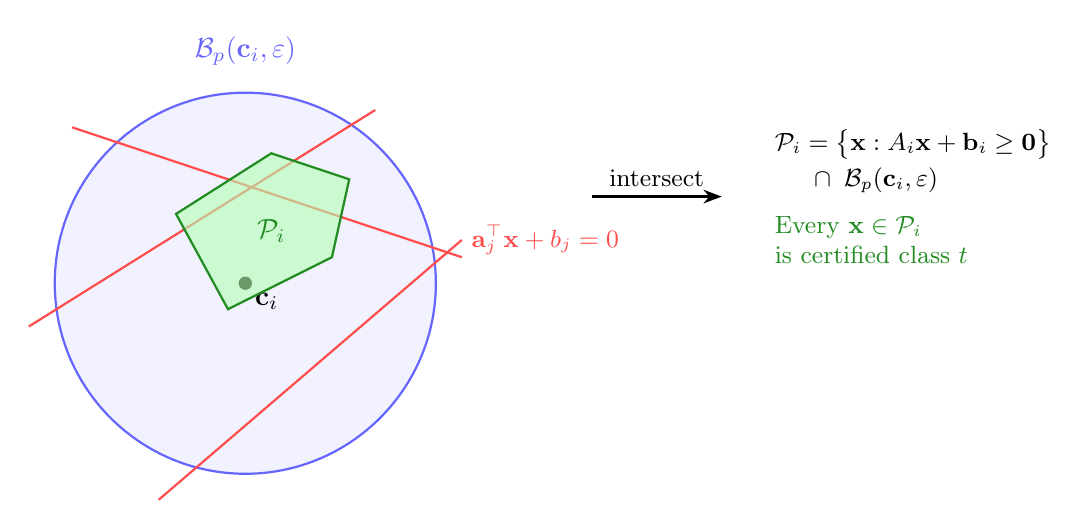
\begin{tikzpicture}[scale=1.1]
  % Epsilon ball
  \draw[thick, blue!60, fill=blue!5] (0,0) circle (2.2cm);
  \node[blue!60, above] at (0, 2.4) {$\Bp(\vc_i, \varepsilon)$};

  % Center point
  \filldraw[black] (0,0) circle (2pt) node[below right] {$\vc_i$};

  % Halfspaces (lines)
  \draw[thick, red!70] (-2.5, -0.5) -- (1.5, 2.0);
  \draw[thick, red!70] (-1.0, -2.5) -- (2.5, 0.5);
  \draw[thick, red!70] (-2.0, 1.8) -- (2.5, 0.3);

  \node[red!70, right] at (2.5, 0.5) {\small $\va_j^\top \vx + b_j = 0$};

  % Certified polytope (intersection)
  \fill[green!30, opacity=0.6] (-0.2, -0.3) -- (1.0, 0.3) -- (1.2, 1.2) -- (0.3, 1.5) -- (-0.8, 0.8) -- cycle;
  \draw[thick, darkgreen] (-0.2, -0.3) -- (1.0, 0.3) -- (1.2, 1.2) -- (0.3, 1.5) -- (-0.8, 0.8) -- cycle;

  \node[darkgreen, font=\bfseries] at (0.3, 0.6) {$\PP_i$};

  % Arrow
  \draw[-{Stealth}, thick] (4, 1) -- (5.5, 1) node[midway, above] {\small intersect};

  % Result description
  \node[right, align=left, font=\small] at (6, 1) {
    $\PP_i = \bigl\{\vx : A_i \vx + \vb_i \geq \mathbf{0}\bigr\}$\\[2pt]
    $\phantom{\PP_i} \;\cap\; \Bp(\vc_i, \varepsilon)$\\[6pt]
    \textcolor{darkgreen}{Every $\vx \in \PP_i$}\\
    \textcolor{darkgreen}{is certified class $t$}
  };
\end{tikzpicture}
\end{center}

\medskip

The \textbf{Certified Atlas} is the collection $\{\PP_i\}_{i=1}^{N_t}$ for all training samples of class~$t$.

\end{frame}

% ================================================================
\section{Efficient Search with BVH}

% ----------------------------------------------------------------
\begin{frame}{BVH Spatial Indexing}

\textbf{Problem:} With $N$ polytopes per class, na\"ive search requires $N$ QP solves per query.\\
In 784 dimensions (MNIST), each QP costs \enquote{a lot} $\Rightarrow$ \textbf{intractable}.

\bigskip

\begin{block}{Bounding Volume Hierarchy (BVH)}
\begin{itemize}
  \item Build a \textbf{binary tree} over polytope bounding boxes
  \item Split along axis of maximum spread (median split)
  \item Each internal node stores the AABB of its children
  \item \textbf{Branch-and-bound} search: prune subtrees whose bounding box is farther than current best
\end{itemize}
\end{block}

\bigskip

\begin{columns}[c]
\column{0.5\textwidth}
\textbf{Complexity:}
\begin{itemize}
  \item Construction: $O(N \log N)$
  \item Query: $O(\log N)$ QP solves
  \item Preserves \textbf{exact} optimality
\end{itemize}

\column{0.5\textwidth}
\textbf{Empirical results (MNIST):}
\begin{itemize}
  \item $\sim$1000 polytopes per class
  \item BVH: $\sim$2--5 QPs per query
  \item vs.\ exhaustive: 1000 QPs
  \item \textbf{$200{-}500\times$ speedup}
\end{itemize}
\end{columns}

\end{frame}

% ----------------------------------------------------------------
\begin{frame}{BVH Branch-and-Bound Search}

\begin{center}
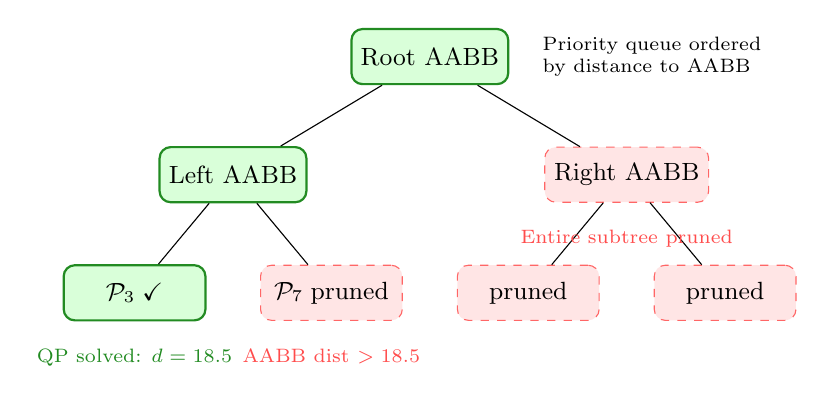
\begin{tikzpicture}[
  node distance=1.2cm,
  every node/.style={draw, rounded corners, minimum width=1.8cm, minimum height=0.7cm, font=\small},
  prune/.style={draw=red!60, fill=red!10, dashed},
  visit/.style={draw=darkgreen, fill=green!15, thick},
  level 1/.style={sibling distance=5cm},
  level 2/.style={sibling distance=2.5cm}
]
  \node[visit] (root) {Root AABB}
    child {
      node[visit] (L) {Left AABB}
      child { node[visit] (LL) {$\PP_3$\;\checkmark} }
      child { node[prune] (LR) {$\PP_7$\;pruned} }
    }
    child {
      node[prune] (R) {Right AABB}
      child { node[prune] (RL) {pruned} }
      child { node[prune] (RR) {pruned} }
    };

  \node[draw=none, right=0.3cm of root, align=left, font=\scriptsize] {
    Priority queue ordered\\by distance to AABB
  };

  \node[draw=none, below=0.1cm of LL, font=\scriptsize, darkgreen] {
    QP solved: $d=18.5$
  };

  \node[draw=none, below=0.1cm of LR, font=\scriptsize, red!70] {
    AABB dist $> 18.5$
  };

  \node[draw=none, below=0.1cm of R, font=\scriptsize, red!70] {
    Entire subtree pruned
  };
\end{tikzpicture}
\end{center}

\medskip

\textbf{Key:} The priority queue ensures we always explore the most promising subtree first.\\
Once we find a good projection, most of the tree is pruned away.

\end{frame}

% ================================================================
\section{$\delta$-Robust Counterfactuals}

% ----------------------------------------------------------------
\begin{frame}{Certified Robustness via Polytope Erosion}

\textbf{Goal:} The counterfactual $\vx'$ should remain valid even under adversarial perturbation of radius~$\delta$.

\begin{block}{$\delta$-Robust Counterfactual}
We want the \textbf{entire ball} $\Bq(\vx', \delta)$ to lie inside the certified polytope $\PP_i$:
\[
  \Bq(\vx', \delta) \subseteq \PP_i \quad\Longrightarrow\quad \text{any perturbation in } \Bq(\vx', \delta) \text{ stays class } t
\]
\end{block}

\medskip

This is achieved by \textbf{eroding} the constraints inward:

\begin{align*}
  \text{Halfspace erosion:}\quad & \va_j^\top \vx + b_j \geq \delta \cdot \|\va_j\|_{q^*}
    & \bigl(\tfrac{1}{q}+\tfrac{1}{q^*}=1\bigr) \\[4pt]
  \text{Ball shrinkage:}\quad & \|\vx - \vc_i\|_p \leq \varepsilon - \delta \cdot \mathcal{C}(q \!\to\! p)
    & \bigl(\mathcal{C}(q\!\to\! p) = d^{\max(0,\,1/p - 1/q)}\bigr) \\[4pt]
  \text{Box shrinkage:}\quad & \|\vx - \vc_i\|_\infty \leq \varepsilon - \delta
\end{align*}

\medskip

Setting $\delta = 0$ recovers the standard (non-robust) formulation.\\
The robustness norm~$q$ can \textbf{differ} from the certification norm~$p$ (cross-norm robustness).

\end{frame}

% ----------------------------------------------------------------
\begin{frame}{Cross-Norm Robustness: Blending Different $L_p$ Norms}

The certification norm~$p$ (atlas) and the robustness norm~$q$ (threat model) can \textbf{differ}. Two mechanisms handle this:

\begin{block}{1. Halfspace erosion via the \textbf{dual norm} $q^*$}
\vspace{-6pt}
To ensure $\Bq(\vx', \delta)$ satisfies $\va_j^\top \vx + b_j \geq 0$, we need:
$\va_j^\top \vx' + b_j \geq \delta \cdot \|\va_j\|_{q^*}$
where $\tfrac{1}{q} + \tfrac{1}{q^*} = 1$.

\smallskip
\emph{Why?} H\"older's inequality: $|\va_j^\top \Delta\vx| \leq \|\va_j\|_{q^*}\|\Delta\vx\|_q \leq \delta\|\va_j\|_{q^*}$.

\smallskip
{\small\begin{tabular}{lccc}
  \toprule
  Robustness norm $q$ & $1$ & $2$ & $\infty$ \\
  \midrule
  Dual $q^*$ & $\infty$ & $2$ & $1$ \\
  Erosion per row & $\max_k|a_{jk}|$ & $\|\va_j\|_2$ & $\sum_k|a_{jk}|$ \\
  \bottomrule
\end{tabular}}
\end{block}

\begin{block}{2. Ball shrinkage via \textbf{norm embedding}}
\vspace{-6pt}
For $p_2 > p_1$: \; $\|\vx\|_{p_2} \leq \|\vx\|_{p_1}$ (free direction), \; but \; $\|\vx\|_{p_1} \leq d^{1/p_1 - 1/p_2}\|\vx\|_{p_2}$ (costly).

\smallskip
If $\Delta\vx \in \Bq(\vx', \delta)$, we must fit it inside $\Bp(\vc_i, \varepsilon)$.
Conversion factor: $\mathcal{C}(q\!\to\!p) = d^{\max(0,\,1/p - 1/q)}$.
\end{block}

\end{frame}

% ----------------------------------------------------------------
\begin{frame}{Norm Ordering and Its Consequences}

\begin{block}{Norm Monotonicity}
For any $\vx \in \R^d$ and $1 \leq p_1 < p_2 \leq \infty$:
\[
  \boxed{\|\vx\|_{p_2} \;\leq\; \|\vx\|_{p_1} \;\leq\; d^{\,1/p_1\,-\,1/p_2}\;\|\vx\|_{p_2}}
\]
\end{block}

\textbf{Consequence for cross-norm robustness:}

\medskip

\begin{columns}[T]
\column{0.48\textwidth}
% Case q < p: The robustness ball is 'smaller' than the atlas ball
\textbf{Case $q < p$ (e.g., $L_2$ robustness on $L_\infty$ atlas):}
\begin{itemize}
  \item $\Bq(\vx', \delta) \subseteq \Bp(\vx', \delta)$ \emph{for free} (left inequality)
  \item Conversion factor $\mathcal{C}(q\!\to\!p) = 1$
  \item The ball constraint barely shrinks
  \item[$\Rightarrow$] \textcolor{darkgreen}{\textbf{Cheap}} -- robustness nearly free
\end{itemize}

\column{0.48\textwidth}
% Case q > p: The robustness ball is 'larger' and must be shrunk
\textbf{Case $q > p$ (e.g., $L_\infty$ robustness on $L_2$ atlas):}
\begin{itemize}
  \item Need right inequality: $\|\Delta\vx\|_p \leq d^{1/p - 1/q}\,\delta$
  \item Conversion factor $\mathcal{C}(q\!\to\!p) = d^{1/p - 1/q} \gg 1$
  \item The ball shrinks \textbf{dramatically} in high $d$
  \item[$\Rightarrow$] \textcolor{highlight}{\textbf{Expensive}} -- rapid feasibility loss
\end{itemize}
\end{columns}

\bigskip

\textbf{Example (MNIST, $d=784$):} $L_2$ robustness on $L_\infty$ atlas ($q<p$) has $\mathcal{C}(2\!\to\!\infty)=1$ (cheap),\\
but $L_2$ robustness on $L_1$ atlas ($q>p$) has $\mathcal{C}(2\!\to\!1) = 784^{1/1 - 1/2} = 28$ (28$\times$ shrinkage).

\end{frame}

% ----------------------------------------------------------------
\begin{frame}{Effect of $\delta$ on Counterfactuals}

\begin{center}
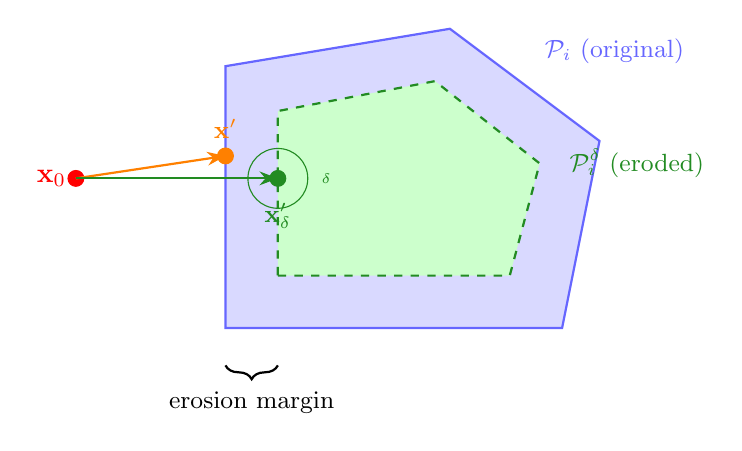
\begin{tikzpicture}[scale=0.95]
  % Original polytope
  \fill[blue!15] (-2,-1.5) -- (2.5,-1.5) -- (3,1) -- (1,2.5) -- (-2,2) -- cycle;
  \draw[thick, blue!60] (-2,-1.5) -- (2.5,-1.5) -- (3,1) -- (1,2.5) -- (-2,2) -- cycle;
  \node[blue!60, font=\small] at (3.2, 2.2) {$\PP_i$ (original)};

  % Eroded polytope
  \fill[green!20] (-1.3,-0.8) -- (1.8,-0.8) -- (2.2,0.7) -- (0.8,1.8) -- (-1.3,1.4) -- cycle;
  \draw[thick, darkgreen, dashed] (-1.3,-0.8) -- (1.8,-0.8) -- (2.2,0.7) -- (0.8,1.8) -- (-1.3,1.4) -- cycle;
  \node[darkgreen, font=\small] at (3.5, 0.7) {$\PP_i^{\delta}$ (eroded)};

  % Query point
  \filldraw[red] (-4, 0.5) circle (3pt) node[left] {$\vx_0$};

  % Standard CF
  \draw[-{Stealth}, thick, orange] (-4, 0.5) -- (-2, 0.8);
  \filldraw[orange] (-2, 0.8) circle (3pt);
  \node[orange, above, font=\small] at (-2, 0.9) {$\vx'$};

  % Robust CF
  \draw[-{Stealth}, thick, darkgreen] (-4, 0.5) -- (-1.3, 0.5);
  \filldraw[darkgreen] (-1.3, 0.5) circle (3pt);
  \node[darkgreen, below, font=\small] at (-1.3, 0.3) {$\vx'_\delta$};
  \draw[darkgreen, thin] (-1.3, 0.5) circle (0.4cm);
  \node[darkgreen, font=\tiny, right] at (-0.85, 0.5) {$\delta$};

  % Annotation
  \draw[decorate, decoration={brace, amplitude=5pt, mirror}, thick]
    (-2, -2) -- (-1.3, -2) node[midway, below=6pt, font=\small] {erosion margin};
\end{tikzpicture}
\end{center}

\medskip

\begin{itemize}
  \item Larger $\delta$ $\Rightarrow$ smaller eroded polytope $\Rightarrow$ farther counterfactual
  \item If $\delta$ is too large, the eroded polytope may become \textbf{empty} (infeasible)
  \item Trade-off: \textbf{proximity vs.\ robustness}
\end{itemize}

\end{frame}

% ================================================================
\section{Experimental Results}

% ----------------------------------------------------------------
\begin{frame}{Experimental Setup}

\begin{columns}[T]
\column{0.48\textwidth}
\textbf{2D Spiral Dataset:}
\begin{itemize}
  \item 5 classes, 80 samples/class (test set)
  \item SimpleClassifier: 2 hidden layers (64, 32)
  \item $\varepsilon = 0.1$, $L_2$ norm
  \item Polytopes directly visualizable
\end{itemize}

\bigskip

\textbf{MNIST Dataset:}
\begin{itemize}
  \item 10 classes, 1000 samples/class
  \item CNN: 4 Conv2d + Linear (99.2\% accuracy)
  \item $\varepsilon = 0.01$, $L_\infty$ norm
  \item 784-dimensional input space
\end{itemize}

\column{0.48\textwidth}
\textbf{Evaluation metrics:}
\begin{itemize}
  \item \textbf{$\ell_2$ distance} (proximity)
  \item \textbf{$\ell_1$ distance / sparsity} (interpretability)
  \item \textbf{LOF score} (plausibility -- closeness to target manifold)
  \item \textbf{QP solves} (computational cost)
  \item \textbf{Validity rate} (must be 100\% by construction)
\end{itemize}

\bigskip

\textbf{Solvers:}
\begin{itemize}
  \item $L_\infty$: SLSQP (all-linear constraints)
  \item $L_2/L_1$: CVXPY + CLARABEL (SOCP)
\end{itemize}
\end{columns}

\end{frame}

% ----------------------------------------------------------------
\begin{frame}{Results: 2D Spiral}

\textbf{Atlas construction:}
\begin{itemize}
  \item 400 polytopes across 5 classes
  \item Feasibility: 48.8\%--90.0\% per class ($\varepsilon=0.1$, $L_2$)
  \item Direct visualization of certified regions possible
\end{itemize}

\bigskip

\textbf{Counterfactual generation:}
\begin{itemize}
  \item 100\% validity rate (all counterfactuals certified)
  \item $\delta$-robust counterfactuals with $\delta = 0.07$, $L_2$ robustness norm
  \item BVH: \textbf{11.6$\times$ fewer QPs} compared to exhaustive search (6.9 vs.\ 80 avg)
\end{itemize}

\bigskip

\textbf{Observations:}
\begin{itemize}
  \item Counterfactuals follow the spiral geometry of the data
  \item Positive margin surplus (min margin $\gg 0$) confirms deep placement inside polytopes
  \item Cross-class distance varies naturally with class separation
\end{itemize}

\end{frame}

% ----------------------------------------------------------------
\begin{frame}{Results: MNIST}

\textbf{Atlas construction:}
\begin{itemize}
  \item 10,000 polytopes across 10 digit classes
  \item $\varepsilon = 0.01$, $L_\infty$ norm $\Rightarrow$ 100\% feasible polytopes
  \item BVH tree depth: 11--12 per class
\end{itemize}

\bigskip

\textbf{Counterfactual generation (digit 1 $\to$ all other digits):}
\begin{itemize}
  \item \textbf{100\% success rate}, 100\% validity (certified by construction)
  \item Average QP solves with BVH: \textbf{1.0--2.7} per query (vs.\ $\sim$1000 exhaustive)
  \item Closest target: digit 7 (avg $\ell_2 = 14.98$), farthest: digit 0 (avg $\ell_2 = 26.20$)
\end{itemize}

\bigskip

\textbf{$\delta$-Robustness (digit 3 $\to$ digit 8):}
\begin{itemize}
  \item $L_\infty$ robustness: stable up to $\delta = 0.1$ (small distance increase)
  \item $L_2$ robustness: feasible up to $\delta = 0.005$ (stricter in 784D due to norm conversion)
\end{itemize}

\end{frame}

% ----------------------------------------------------------------
\begin{frame}{Quality Metrics (MNIST, 180 Counterfactuals)}

\begin{center}
\begin{tabular}{lrr}
  \toprule
  \textbf{Metric} & \textbf{Mean} & \textbf{Median} \\
  \midrule
  $\ell_2$ distance           & 23.4  & 22.8  \\
  $\ell_\infty$ distance      & 3.22  & 3.22  \\
  $\ell_1$ distance           & 322.8 & 307.0 \\
  Pixels changed (of 784)     & 224   & 221   \\
  Sparsity (\% pixels changed)& 28.6\%& 28.2\% \\
  LOF score                   & 1.55  & 1.29  \\
  QP solves (BVH)             & 3.4   & 2.0   \\
  \bottomrule
\end{tabular}
\end{center}

\bigskip

\begin{itemize}
  \item \textbf{LOF $\approx$ 1} indicates counterfactuals are plausible (close to inliers in target class)
  \item \textbf{$\sim$29\% of pixels changed} -- counterfactuals are moderately sparse
  \item \textbf{BVH reduces QP solves by $\sim$300$\times$} compared to exhaustive search
\end{itemize}

\end{frame}

% ================================================================
\section{Summary \& Next Steps}

% ----------------------------------------------------------------
\begin{frame}{Summary}

\begin{block}{Contributions}
\begin{enumerate}
  \item \textbf{Certified Polyhedral Projection (CPP)} -- transforms CE generation from non-convex optimization into a series of convex QP projections
  \item \textbf{Provable validity} -- counterfactuals lie inside LiRPA-certified polytopes $\Rightarrow$ guaranteed target-class prediction
  \item \textbf{$\delta$-robust counterfactuals} -- polytope erosion ensures certified robustness to adversarial perturbations, with support for cross-norm robustness
  \item \textbf{BVH spatial indexing} -- enables $O(\log N)$ search instead of $O(N)$, achieving $200{-}500\times$ speedup on MNIST
\end{enumerate}
\end{block}

\bigskip

\begin{block}{Key Properties}
\begin{itemize}
  \item \textbf{No hyperparameter $\lambda$} -- proximity is handled by projection, validity by certification
  \item \textbf{Global optimality per polytope} -- convex QP guarantees
  \item \textbf{Offline/online separation} -- atlas built once, queries are fast
\end{itemize}
\end{block}

\end{frame}

% ----------------------------------------------------------------
% \begin{frame}{Next Steps}

% \begin{enumerate}
%   \item \textbf{Tighter bounds} -- use $\alpha$-CROWN or multi-step bound tightening to increase polytope volume and feasibility at larger $\varepsilon$

%   \item \textbf{Scalability} -- extend to higher-resolution images (CIFAR-10, ImageNet) with improved batch LiRPA computation

%   \item \textbf{Latent-space CPP} -- apply polytope construction in a learned latent space (e.g., VAE encoder) for more natural counterfactuals

%   \item \textbf{Sparsity regularization} -- add $\ell_1$ penalties to the QP objective for sparser, more interpretable counterfactuals

%   \item \textbf{Comparison with baselines} -- systematic benchmarking against DiCE, FACE, Growing Spheres, and other CE methods

%   \item \textbf{Actionability constraints} -- incorporate domain-specific constraints (e.g., monotonicity, immutability) into the QP formulation
% \end{enumerate}

% \end{frame}

% ----------------------------------------------------------------
\begin{frame}

\begin{center}
  {\Huge\textcolor{darkblue}{Thank You}}

  \bigskip

  {\large Questions?}

  \bigskip\bigskip

  \texttt{github.com/gabrielepintus/PreimageCounterfactualSampling}
\end{center}

\end{frame}

\end{document}
